\documentclass[12pt,a4paper,]{report}
\usepackage{lmodern}

% Overwrite \begin{figure}[htbp] with \begin{figure}[H]
\usepackage{float}
\let\origfigure=\figure
\let\endorigfigure=\endfigure
\renewenvironment{figure}[1][]{%
\origfigure[b]
}{%
\endorigfigure
}

% fix for pandoc 1.14
\providecommand{\tightlist}{%
  \setlength{\itemsep}{0pt}\setlength{\parskip}{0pt}}

% TP: hack to truncate list of figures/tables.
\usepackage{truncate}
\usepackage{caption}
\usepackage{tocloft}
% TP: end hack

\usepackage{amssymb,amsmath}
\usepackage{ifxetex,ifluatex}
\usepackage{fixltx2e} % provides \textsubscript
\ifnum 0\ifxetex 1\fi\ifluatex 1\fi=0 % if pdftex
  \usepackage[T1]{fontenc}
  \usepackage[utf8]{inputenc}
\else % if luatex or xelatex
  \ifxetex
    \usepackage{mathspec}
    \usepackage{xltxtra,xunicode}
  \else
    \usepackage{fontspec}
  \fi
  \defaultfontfeatures{Mapping=tex-text,Scale=MatchLowercase}
  \newcommand{\euro}{€}
\fi
% use upquote if available, for straight quotes in verbatim environments
\IfFileExists{upquote.sty}{\usepackage{upquote}}{}
% use microtype if available
\IfFileExists{microtype.sty}{%
\usepackage{microtype}
\UseMicrotypeSet[protrusion]{basicmath} % disable protrusion for tt fonts
}{}
\usepackage{graphicx}
\makeatletter
\def\maxwidth{\ifdim\Gin@nat@width>\linewidth\linewidth\else\Gin@nat@width\fi}
\def\maxheight{\ifdim\Gin@nat@height>\textheight\textheight\else\Gin@nat@height\fi}
\makeatother
% Scale images if necessary, so that they will not overflow the page
% margins by default, and it is still possible to overwrite the defaults
% using explicit options in \includegraphics[width, height, ...]{}
\setkeys{Gin}{width=\maxwidth,height=\maxheight,keepaspectratio}
\ifxetex
  \usepackage[setpagesize=false, % page size defined by xetex
              unicode=false, % unicode breaks when used with xetex
              xetex]{hyperref}
\else
  \usepackage[unicode=true]{hyperref}
\fi
\hypersetup{breaklinks=true,
            bookmarks=true,
            pdfauthor={},
            pdftitle={},
            colorlinks=true,
            citecolor=blue,
            urlcolor=blue,
            linkcolor=magenta,
            pdfborder={0 0 0}}
\urlstyle{same}  % don't use monospace font for urls
\setlength{\parindent}{0pt}
\setlength{\parskip}{6pt plus 2pt minus 1pt}
\setlength{\emergencystretch}{3em}  % prevent overfull lines
\setcounter{secnumdepth}{5}

\date{}


% Table of contents formatting
\renewcommand{\contentsname}{Table of Contents}
\setcounter{tocdepth}{3}

% Headers and page numbering
\usepackage{fancyhdr}
\pagestyle{plain}

% Following package is used to add background image to front page
\usepackage{wallpaper}

% Table package
\usepackage{ctable}% http://ctan.org/pkg/ctable

% Deal with 'LaTeX Error: Too many unprocessed floats.'
\usepackage{morefloats}
% or use \extrafloats{100}
% add some \clearpage

% % Chapter header
% \usepackage{titlesec, blindtext, color}
% \definecolor{gray75}{gray}{0.75}
% \newcommand{\hsp}{\hspace{20pt}}
% \titleformat{\chapter}[hang]{\Huge\bfseries}{\thechapter\hsp\textcolor{gray75}{|}\hsp}{0pt}{\Huge\bfseries}

% % Fonts and typesetting
% \setmainfont[Scale=1.1]{Helvetica}
% \setsansfont[Scale=1.1]{Verdana}

% FONTS
\usepackage{xunicode}
\usepackage{xltxtra}
\defaultfontfeatures{Mapping=tex-text} % converts LaTeX specials (``quotes'' --- dashes etc.) to unicode
% \setromanfont[Scale=1.01,Ligatures={Common},Numbers={OldStyle}]{Palatino}
% \setromanfont[Scale=1.01,Ligatures={Common},Numbers={OldStyle}]{Adobe Caslon Pro}
%Following line controls size of code chunks
% \setmonofont[Scale=0.9]{Monaco}
%Following line controls size of figure legends
% \setsansfont[Scale=1.2]{Optima Regular}

%Attempt to set math size
%First size must match the text size in the document or command will not work
%\DeclareMathSizes{display size}{text size}{script size}{scriptscript size}.
\DeclareMathSizes{12}{13}{7}{7}

% ---- CUSTOM AMPERSAND
% \newcommand{\amper}{{\fontspec[Scale=.95]{Adobe Caslon Pro}\selectfont\itshape\&}}

% HEADINGS
\usepackage{sectsty}
\usepackage[normalem]{ulem}
\sectionfont{\rmfamily\mdseries\Large}
\subsectionfont{\rmfamily\mdseries\scshape\large}
\subsubsectionfont{\rmfamily\bfseries\upshape\large}
% \sectionfont{\rmfamily\mdseries\Large}
% \subsectionfont{\rmfamily\mdseries\scshape\normalsize}
% \subsubsectionfont{\rmfamily\bfseries\upshape\normalsize}

% Set figure legends and captions to be smaller sized sans serif font
\usepackage[font={footnotesize,sf}]{caption}

\usepackage{siunitx}

% Adjust spacing between lines to 1.5
\usepackage{setspace}
\onehalfspacing
% \doublespacing
\raggedbottom

% Set margins
\usepackage[top=1.5in,bottom=1.5in,left=1.5in,right=1.4in]{geometry}
% \setlength\parindent{0.4in} % indent at start of paragraphs (set to 0.3?)
\setlength{\parskip}{9pt}

% Add space between pararaphs
% http://texblog.org/2012/11/07/correctly-typesetting-paragraphs-in-latex/
% \usepackage{parskip}
% \setlength{\parskip}{\baselineskip}

% Set colour of links to black so that they don't show up when printed
\usepackage{hyperref}
\hypersetup{colorlinks=false, linkcolor=black}

% Tables
\usepackage{booktabs}
\usepackage{threeparttable}
\usepackage{array}
\newcolumntype{x}[1]{%
>{\centering\arraybackslash}m{#1}}%

% Allow for long captions and float captions on opposite page of figures
% \usepackage[rightFloats, CaptionBefore]{fltpage}

% Don't let floats cross subsections
% \usepackage[section,subsection]{extraplaceins}

\begin{document}

\begin{titlepage}
    \begin{center}
        
        \vspace*{2.5cm}
        
        \huge
        Is occupational asbestos exposure an under-recognised cause of idiopathic pulmonary fibrosis?
        \vspace{1.5cm}
        
        \Large
        Carl Jonathan Reynolds
        
        \vspace{1.5cm}

        \normalsize
        A thesis presented for the degree of\\
        Doctor of Philosophy
        
        \vfill
        
        \normalsize
        Supervised by:\\
        Professor Paul Cullinan\\
        Dr Chris Barber \\
        Dr Sara De Matteis

        \vspace{0.8cm}

        \normalsize
        Imperial College London, UK\\
        January 2018

         Except where otherwise noted, content in this thesis is licensed under a Creative Commons Attribution 4.0 License (http://creativecommons.org/licenses/by/4.0), which permits unrestricted use, distribution, and reproduction in any medium, provided the original work is properly cited. Copyright 2018, Carl Reynolds.

    \end{center}
\end{titlepage}

\vspace*{\fill}

\noindent \textit{
I, Carl Jonathan Reynolds confirm that the work presented in this thesis is my own. Where information has been derived from other sources, I confirm that this has been indicated in the thesis.
} \vspace*{\fill} \pagenumbering{gobble}

\hypertarget{abstract}{%
\chapter*{Abstract}\label{abstract}}
\addcontentsline{toc}{chapter}{Abstract}

The question of whether occupational asbestos exposure is an
under-recognized cause of idiopathic pulmonary fibrosis arises because
it is clinically plausible, epidemiologically plausible, and consistent
with fibre studies and case-control data. This thesis examines the
question by means of a literature review and a novel hospital based
case-control study, the idiopathic pulmonary fibrosis job exposures
study (IPFJES).

\pagenumbering{roman}
\setcounter{page}{1}

\hypertarget{acknowledgements}{%
\chapter*{Acknowledgements}\label{acknowledgements}}
\addcontentsline{toc}{chapter}{Acknowledgements}

I am grateful to Zeinab, Ada, and Rosa for putting up with me.

I am grateful to Paul, Chris, and Sara for their supervision.

I am grateful to the partcipants, to Rupa and all of the principle
investigators and their teams for making the study happen.

\newpage

\pagenumbering{gobble}

\tableofcontents

\newpage

\hypertarget{list-of-figures}{%
\chapter*{List of figures}\label{list-of-figures}}
\addcontentsline{toc}{chapter}{List of figures}

Figure 4.1 This is an example figure . . . \hfill{pp}\\
Figure x.x Short title of the figure . . . \hfill{pp}

\pagenumbering{roman}
\setcounter{page}{3}

\newpage

\hypertarget{list-of-tables}{%
\chapter*{List of tables}\label{list-of-tables}}
\addcontentsline{toc}{chapter}{List of tables}

Table 5.1 This is an example table . . . \hfill{pp}\\
Table x.x Short title of the figure . . . \hfill{pp}

\hypertarget{abbreviations}{%
\chapter*{Abbreviations}\label{abbreviations}}
\addcontentsline{toc}{chapter}{Abbreviations}

\begin{itemize}
\tightlist
\item
  \textbf{IPF} Idiopathic pulmonary fibrosis.
\item
  \textbf{MUC5B} Mucin 5B gene.
\end{itemize}

\newpage
\setcounter{page}{1}
\renewcommand{\thepage}{\arabic{page}}

\hypertarget{introduction-to-thesis}{%
\chapter{Introduction to thesis}\label{introduction-to-thesis}}

\hypertarget{occupational-asbestos-exposure-as-an-underecognised-cause-of-idiopathic-pulmonary-fibrosis}{%
\section{Occupational asbestos exposure as an underecognised cause of
idiopathic pulmonary
fibrosis}\label{occupational-asbestos-exposure-as-an-underecognised-cause-of-idiopathic-pulmonary-fibrosis}}

Idiopathic pulmonary fibrosis (IPF) is a progressive, fibrotic lung
disease which in 2012 was the recorded cause of death for c.4000 people
in England and Wales. Its incidence, currently around 7.5/100,000
person-years, has increased by 5\% pa since 2000.{[}1{]} The
pathophysiology of IPF is complex, the outcome of host susceptibility
factors, epithelial injury, and a dysregulated repair process. Several
gene polymorphisms which result in a vulnerable alveolar epithelium have
been characterized; they include abnormalities in mucin genes (eg
MUC5B), surfactant protein genes, and telomerase genes (eg TERT and
TERC).{[}2{]}{[}3{]}{[}4{]} The median age of onset is 70 years and the
condition is more common in men (M:F ratio 1.6), manual workers, and
those living in industrial areas{[}1{]}, patterns that are not unique to
the UK.{[}3{]} The prognosis is poor, with a median survival of three
years.{[}5{]}{[}6{]}

These epidemiological distributions of IPF are consistent with a
long-latency response to occupational dust exposure; in particular, the
incidence of IPF correlates strongly (if ecologically) with historic
asbestos use.{[}7{]} Mineralogical studies support the concept of
asbestosis-IPF misclassification by revealing high fibre burdens in the
lung tissue of patients diagnosed with `IPF' and revision of the
diagnosis to `asbestosis'.{[}8{]}{[}9{]}{[}10{]}{[}11{]}

Identification of occupational asbestos fibre exposure as an
under-recognised cause of IPF is important to improve our understanding
of the aetio-pathophysiology of IPF and the accuracy of prognostic
information. It would have implications for compensation and impact on
the current restrictions on individual treatment. Importantly, it would
inform evidence-based workplace exposure policies in the UK and
internationally, particularly in the many countries with continuing high
levels of asbestos use.

\hypertarget{aims-and-objectives}{%
\section{Aims and objectives}\label{aims-and-objectives}}

My overall aim is to characterize and measure asbestos exposure as an
occupational determinant of IPF; additionally, I will determine
host-exposure interactions mediated by candidate susceptibility
polymorphisms (in particular MUC5B promoter polymorphism rs35705950).

My specific research questions are:

\begin{enumerate}
\def\labelenumi{\arabic{enumi}.}
\tightlist
\item
  Does a dose-response relationship exist for occupational asbestos
  exposure and IPF?
\item
  Does the presence of asbestos exposure modify the association between
  IPF and rs35705950?
\end{enumerate}

\hypertarget{data-sources}{%
\section{Data sources}\label{data-sources}}

\begin{itemize}
\tightlist
\item
  For the literature review and meta-analysis of occupational exposures
  in IPF I consider all published IPF case-control studies reporting on
  occupational exposures.
\item
  For the mortality analysis I use data obtained from the Office of
  National Statistics, Health and Safety Executive, and the World Health
  Organisation Mortality Database.
\item
  Brief reviews of asbestos exposure assessment and genetic
  suceptibility in IPF rely on the published literature.
\item
  Primary case-control data collected during my PhD as part of the
  idiopathic pulmonary fibrosis job exposures study (IPFJES) is used to
  analyze asbestos exposure in IPF. (?include navaratum case control
  jobs data that was shared)
\end{itemize}

\hypertarget{outline-of-thesis}{%
\section{Outline of thesis}\label{outline-of-thesis}}

This chapter (Chapter 1) describes the problem studied, aims and
objectives, and approach. Chapter 2 is a literature review and
meta-analysis of IPF case-control studies that report on occupational
exposure. Chapter 3 is an analysis of IPF and asbestos related disease
mortality data. Chapter 4 is a review of asbestos exposure assessment
methodology. Chapter 5 is a review of genetic suceptibility in IPF.
Chapter 6 describes the idiopathic pulmonary fibrosis job exposures
study including results and analysis arising from it. Chapter 7
concludes the thesis by summarising it and suggesting future work.

\hypertarget{literature-review-and-meta-analysis-how-much-ipf-is-attributable-to-occupational-exposures}{%
\chapter{Literature review and meta-analysis: how much IPF is
attributable to occupational
exposures?}\label{literature-review-and-meta-analysis-how-much-ipf-is-attributable-to-occupational-exposures}}

\hypertarget{introduction}{%
\section{Introduction}\label{introduction}}

Idiopathic pulmonary fibrosis (IPF) is a diagnosis of exclusion. It is
made in the presence of a usual interstitial pneumonitis (UIP) pattern
on high resolution CT scan or biopsy. The diagnosis requires that known
causes of interstitial lung disease (such as drug toxicity, connective
tissue disease, domestic, and occupational or environmental exposures)
be excluded.{[}12{]}

Attributing a disease process to a specific exposure can be difficult.
Disease processes are frequently complex or multifactorial, depending on
the interaction of genetic and environmental components. Well-studied
and relatively frequent entities such as chronic obstructive pulmonary
disease, ischaemic heart disease and diabetes lend themselves to
epidemiologic investigation, delineating the major risk factors for
disease and their relative contributions to risk at the population
level. IPF presents an additional challenge to attribution; because of
its relative infrequency, epidemiologic study of the disease is largely
limited to case-control studies.{[}13{]} Studying specific occupational
exposures also presents its own challenges; co-exposure is common,
occupational hygeine data is frequently limited and self-reported
exposure is prone to recall bias.

I identified several review articles of the epidemiology of interstitial
lung disease that do not necessarily focus on IPF and only briefly
mention occupational factors (e.g Ley2013{[}3{]}). Here I consider
review articles that specifically deal with occupational factors in IPF
and cite the case-control studies used.

Turner-Warwick (1998) discusses potential difficulties in establishing
attribution and causality in IPF. She observes that there is variation
in clinical practice with respect to the standard applied to exclude
IPF; some clinicians exclude IPF when exposure to a potential cause is
identified, others only when there is clear exposure to an established
cause. She explains that diagnosis based on radiologic and clinical
findings, and not on lung biopsy or bronchioalveolar lavage, may result
in initiating agents for disease being overlooked. Further, that
exposures such as asbestos, silica, coal, graphite, hard metal, and
avian proteins, may result in disease that can not be differentiated
from IPF.{[}14{]}

Reviewing the epidemiology of IPF and case-control studies to date
Hubbard (2001) describes the association of IPF with occupational
exposures to metal and wood and estimates that 10\% of IPF cases may be
due to occupational metal exposure and 5\% of cases to wood.{[}15{]}

Taskar and Coultas (2006) review and carry out a meta-analysis of six
case-control studies investigating environmental and occupational
exposures in IPF. They report population attributable risk percentages
for agriculture and farming (20.8\%), livestock (4.1\%), wood dust
(5\%), metal dust (3.4\%), stone/sand/silica (3.5\%), and smoking
(49.1\%).{[}16{]}

Gulati and Redlich's (2015) review of exposures causing usual
interstitial pneumonia highlights that asbestosis may appear
indistinguishable from IPF and summarises previous case-control studies
but did not pool studies to perform a meta-analysis.{[}17{]}

I sought to identify and meta-analyze all IPF case-control studies
dealing with occupational exposures.

\hypertarget{method}{%
\section{Method}\label{method}}

Pubmed, embase, and google scholar search engines were searched for
combinations of the terms `idiopathic pulmonary fibrosis', `occupation',
`case-control study' and synonyms. When a relevant papers was identified
papers referenced and papers citing the paper were reviewed. Medline
ranker{[}18{]} and bespoke pubmed `mining' techniques{[}19{]} were also
used.

Two investigators independently reviewed and abstracted data for five
exposure categories common to the identified case-control studies:
``vapors, gases, dusts, and/or fumes (VGDF)'', ``metal dust'', ``wood
dust'', ``silica dust'', and ``agricultural dust''. We calculated PAF as
follows: PAF=pc(OR - 1)/OR, where pc is the proportion of cases exposed
and OR is the risk estimate.

We calculated pooled OR and pooled PAF for occupational exposures using
fixed effects models and random effects models in Stata. When there was
results of the models differed substantively, we used the results of the
fixed effects model, which were more conservative. The pooled PAF relied
on the ratio of attributable cases to all cases underlying each risk
estimate.

\hypertarget{results}{%
\section{Results}\label{results}}

We found (as of May 2017) 15 case-control studies looking at
occupational exposures in IPF the most recent review article covers only
eight of them. Associations with metal, wood, silica, and agricultural
dust were reported. {[}20{]} {[}21{]} {[}22{]} {[}23{]} {[}24{]}
{[}25{]} {[}26{]} {[}27{]} {[}28{]} {[}29{]} {[}30{]} {[}31{]} {[}32{]}
{[}33{]} {[}34{]}

40 risk estimates from 12 publications (1326 IPF cases in total) were
used (Table 3.1){[}20{]} {[}22{]} {[}23{]} {[}24{]} {[}25{]} {[}26{]}
{[}27{]} {[}29{]} {[}30{]} {[}31{]} {[}32{]} {[}34{]}

Three studies were not used, one because data was not collected on the
proportion of cases with specific occupational exposures{[}21{]}, one
because of methodological differences in exposure assignment{[}28{]},
and one because if reported data for pulmonary fibrosis rather than
IPF.{[}33{]}

Each exposure category was assessed with 6-11 risk estimates (Table
3.2).

\begin{table}[htbp]\centering
\caption{Summary of IPF case-control studies investigating occupational exposures}
\label{metatable1}
\small
    \begin{tabular}{|p{1.5cm}|p{0.5cm}p{0.5cm}p{0.5cm}p{0.5cm}p{0.5cm}|p{0.5cm}p{0.5cm}p{0.5cm}p{0.5cm}p{0.5cm}|p{2.5cm}|p{2cm}|}
\midrule
\textbf{Reference (n cases)} & \multicolumn{5}{c}{\textbf{OR; 95\% CI}} & \multicolumn{5}{c}{\textbf{PAF \%}}  \\
        & vgdf* & metal & wood & ag & si & vgdf* & metal & wood & ag & si  \\
\toprule
        Scott 1990(40)\cite{Scott1990}                   & 1.3; 0.8, 2.0 & 11.0; 2.3, 52.4 & 2.9; 0.9, 9.9 & 10.9; 1.2, 96.0 & 1.6; 0.5, 4.8 & 17 & 12 & 10 & 12 & 5   \\
\hline

        Hubbard 1996(218)\cite{Hubbard1996a}                 &               & 1.7; 1.1, 2.7   & 1.7; 1.0, 2.9   &               &   &  & 10  & 6   &  &\\
\hline
        Mullen 1998(15)\cite{Mullen1998}                   & 2.4; 0.7, 8.4   &               & 3.3; 0.4, 25.8  &  & 11; 1.1, 115             & 20 &    & 7  &    & 20                         \\
\hline
        Baumgartner 2000(248)\cite{Baumgartner2000}             &               & 2.0; 1.0, 4.0   & 1.6; 0.8, 3.3   & 1.6; 1.0, 2.5   & 3.9; 1.2, 12.7 &   & 5  & 3  & 7 & 2                \\
\hline
        Hubbard 2000(22)\cite{Hubbard2000}                  &               & 1.1; 0.4, 2.7   &               &               &    &   & 5   &    &  &     \\
\hline
        Miyake 2005(102)\cite{Miyake2005}                  &  5.6; 2.1, 17.9    & 9.6; 1.7, 181.1 & 6.0; 0.3, 112.4 & 0.6; 0.2, 1.9   & 1.8; 0.5, 7.0           & 26 & 11 & 4  & 0   &  5                  \\
\hline
        Gustafson 2007(140)\cite{Gustafson2007}               & 1.1; 0.7, 1.7   & 0.9; 0.5, 1.6   & 1.2; 0.7, 2.2   &   & 1.4; 0.7, 2.7           & 6  & 0   & 3  &    & 3                   \\
\hline
        Garcia-Sancho Figueroa 2010(97)\cite{Garcia-SanchoFigueroa2010}   & 1.2; 0.8, 1.9   &               &               &               &   & 9   &    &    & &                  \\
\hline
        Garcia-Sancho 2011(100)\cite{Garcia-Sancho2011}           & 2.8; 1.5, 5.5   &               &               &               &   &  50  &    &    & &                         \\
\hline
        Awadalla 2012 men (95)\cite{Awadalla2012}                &               & 1.6; 0.7, 3.6   & 2.7; 1.1, 6.8    & 1.0; 0.4, 2.3   & 1.1; 0.5, 2.7 &   & 6  & 9  & 0  & 1                         \\
\hline
        Awadalla 2012 women (106)\cite{Awadalla2012}                &               &    & 4.3; 0.8, 22.1    & 3.3; 1.2, 10.1  & &   &   & 6  & 14  &             \\
\hline
        Paolocci 2013 soft wood (abstract only)(65)\cite{Paolocci2013} &               &     2.8; 1.1, 7.2       & 1.1; 0.4, 3.3 &   & 2.0; 0.9, 4.4               &   &  9  & 0  &    & 11 \\
\hline

        Paolocci 2013 hard wood (abstract only)(n/a)\cite{Paolocci2013} &               &                        &  0.9; 0.3, 2.8    &       &               &   &    &  0 &    &        \\
\hline
        Koo 2017(78)\cite{Koo2017}                      & 2.7; 0.7, 10.9  & 5.0; 1.4, 18.2  & 2.5; 0.5, 12.3  & & 1.2; 0.4, 3.8              & 35 & 22 & 5  &    & 5     \\        
\bottomrule             
\end{tabular}
\end{table}

\hypertarget{discussion}{%
\chapter{Discussion}\label{discussion}}

Our results support the case for a proportion of IPF cases being
attributable to occupational exposures.

Pooled ORs were significantly elevated for VGDF, metal dust, wood dust,
agricultural dust, and silica dust; the pooled PAF estimates by category
ranged from 4-23\%. This is an important finding for an otherwise
idiopathic disease which carries significant morbidity and mortality;
identifying causal occupational agents would permit remidiation and
prevention.

Associations between IPF and wood, metal, and agricultural dust were
previouly reported in a meta-analysis of six case-control studies by
Taskar and Coultas. {[}16{]} While our findings are similar we found a
smaller effect size for agricultural exposure and a large effect size
for non-specific vapours, gases, dust, and fumes (VGDF), see Table 3.2.

Funnel plot asymmetry using Egger's test, which may be due to
publication bias, was present for VGDF (p = 0.04) and metal dust (p =
0.03) but not for wood dust (p = 0.09), silica dust (p = 0.2), and
agricultural dust (p = 0.6). However, the number of studies included is
small and funnel plot assymetry may be due to chance rather than bias.

There are several limitations to the meta-analysis that arise from the
case-control studies included.

Several studies {[}20{]} {[}35{]} {[}24{]} {[}27{]} {[}30{]} used
population controls but do not provide details on participation rates.
Participation rates can be low for community controls; a recent UK
case-control study investigating prothrombotic factors in IPF reported a
response rate of 28\% for commumnity controls. {[}36{]} This approach is
vulnerable to non-responder bias. One study{[}25{]} used employee
occupational records and death certificates from pension-fund records
for a single company and was only able to locate the occupational
records for 40\% of cases and 38\% of controls.

Nearly all studies relied on self-reported exposures rather than life
time occupational histories to assess exposure; an approach that is
prone to recall bias and does not permit examination of dose-response
relationships.

Reliance of self-reported exposures also means that studies are
potentially vulnerable to confounding as a result of co-exposure. For
example, several studies have described strong associations between
metal work and IPF and specify sheet metal
workers{[}21{]}{[}20{]}{[}25{]}, a group who are frequently exposed to
dust containing asbestos fibres{[}37{]} and who in a recent UK study,
had the highest risk of mesothelioma.{[}38{]}

Case definitions and sources for cases varied between studies. For
example Scott (1990){[}20{]} used a case definition which included a
chest radiograph showing bilateral interstitial shadowing whereas most
other studies relied on high resolution CT. Four studies used mortality
data {[}21{]}{[}28{]}{[}27{]}{[}25{]} to identify cases and one
study{[}27{]} used a national register of patients recieving oxygen
therapy. Differences in healthcare coverage and coding practices can
result in selection bias.{[}39{]}

\hypertarget{conclusion}{%
\section{Conclusion}\label{conclusion}}

The observed excess risk could represent disease misclassification of
pneumoconiosis or hypersensitivity pneumonitis, but this is unlikely to
fully explain the observed effects. Our analysis supports an etiologic
role for occupational exposures in IPF, potentially explaining up to
23\% of the burden of disease and highlighting a role for workplace
exposure reduction in disease prevention.

\hypertarget{mortality-analysis-do-mortality-trends-support-an-occupational-cause}{%
\chapter{Mortality analysis: do mortality trends support an occupational
cause?}\label{mortality-analysis-do-mortality-trends-support-an-occupational-cause}}

\hypertarget{introduction-1}{%
\section{Introduction}\label{introduction-1}}

The incidence of Idiopathic pulmonary fibrosis (IPF) has been increasing
at a rate of 5\% per annum since 2000. By definition, the diagnosis of
IPF is not made in the presence of an identifiable cause. However, the
distribution of the disease in the population (more common in men,
manual workers, and those living in more industrial areas of the
country) suggests a causal contribution from an occupational or
environmental source.

It is hypothesised that a proportion of Idiopathic Pulmonary Fibrosis
(IPF) cases are due to occult environmental or occupational exposures to
asbestos dust. This would be expected to result in a spatio-temporal
association between IPF, Mesothelioma, and Asbestosis mortality patterns
coinciding with asbestos exposure. It would also be expected to produce
a birth cohort effect.

Our aim was to examine trends in IPF, Mesothelioma, and Asbestosis
mortality data for evidence of cohort effect and association.

\hypertarget{method-1}{%
\section{Method}\label{method-1}}

Regional age and sex stratified mortality data for IPF, Mesothelioma,
and Asbestosis were obtained for England and Wales from the Office of
National Statistics for the period 1974--2012. Data were
age-standardised and visualised using the Python Pandas data analysis
library and matplotlib.

\hypertarget{results-1}{%
\section{Results}\label{results-1}}

IPF mortality continues to rise. Female:Male is approximately 1:1.6.
There are more IPF deaths in the North West and South East of England.
IPF mortality does appear to correlate with mesothelioma mortality
(Figure \ref{mortalitytrends}). There is evidence of a cohort effect
with age-specific IPF death rates increasing in successive cohorts, most
clearly seen from age 60 (Figure \ref{birthcohorts}). While overall
rates were higher for men but there were not marked sex differences in
cohort mortality trends.

\begin{figure}
\centering
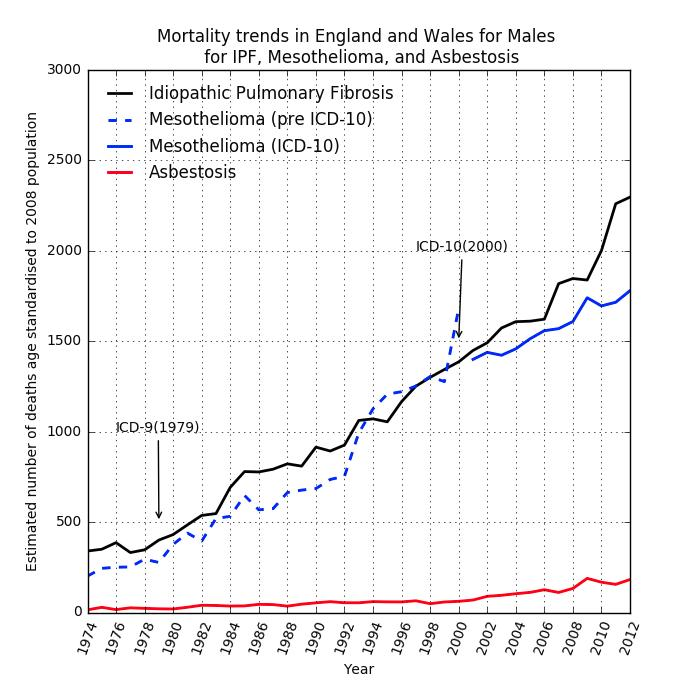
\includegraphics[width=0.5\textwidth,height=\textheight]{./tex2pdf.-c788ce828caea25c/eeadfd2a881431b65eafbc89d9e56a4112d53a37.jpg}
\caption{IPF, mesothelioma, and asbestosis mortality trends
\label{mortalitytrends}}
\end{figure}

\begin{figure}
\centering
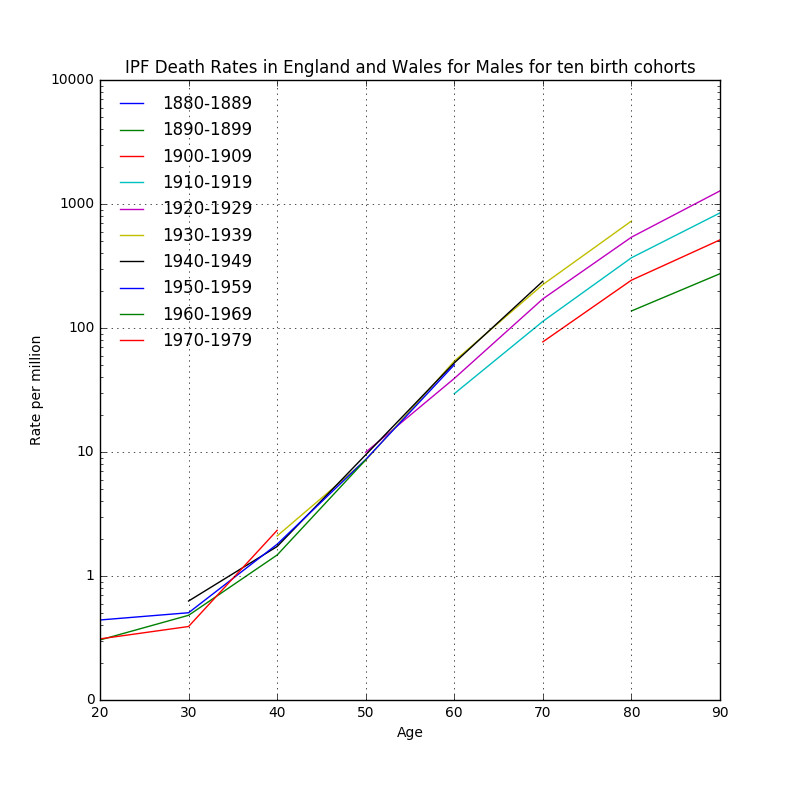
\includegraphics[width=0.5\textwidth,height=\textheight]{./tex2pdf.-c788ce828caea25c/9a5e429b5393b4c4d41e95eeebdd7dc75dc9dab5.jpg}
\caption{IPF male birth cohorts \label{birthcohorts}}
\end{figure}

\hypertarget{discussion-1}{%
\section{Discussion}\label{discussion-1}}

icd coding chat

This is the discussion. Duis ultrices tempor sem vitae convallis.
Pellentesque lobortis risus ac nisi varius bibendum. Phasellus volutpat
aliquam varius. Mauris vitae neque quis libero volutpat finibus. Nunc
diam metus, imperdiet vitae leo sed, varius posuere orci.

\hypertarget{conclusion-1}{%
\section{Conclusion}\label{conclusion-1}}

Conclusions: The birth cohort effect we observed is consistent with a
proportion of IPF cases being due to an occupational or environmental
exposure with latency and further research is needed.

\hypertarget{historic-asbestos-exposure-assessment-can-it-be-done}{%
\chapter{Historic asbestos exposure assessment: can it be
done?}\label{historic-asbestos-exposure-assessment-can-it-be-done}}

\hypertarget{introduction-2}{%
\section{Introduction}\label{introduction-2}}

Asbestos related respiratory disease is initiated by inhalation of
asbestos fibres. In the UK clinically significant asbestos exposure is
largely occupational and, as a result of asbestos control legislation,
historic.

Occupational asbestos exposure can be assessed quantitatively by
sampling ambient air at a workplace and calculating a fibre count using
microscopy. Alternatively, because inhaled asbestos fibres persist in
the lung they can be sampled by lung biopsy, bronchoalveolar lavage, or
at autopsy.

Historic workplace measurements are a valuable resource for assessing
exposure but are limited in several ways. Measurements are not available
for many occupations, where measurements are available they are
dependant on working practices and measurement technique at the time of
assessment; they do not necessarily generalize well.

Measurement of asbestos fibres in lung tissue by means of biopsy or
bronchoalveolar lavage is invasive and both procedures carry the risk of
serious complication including death. Additionally, the biopersistance
of asbestos fibres is variable, counts are sensitive to techniques used,
and establishing appropriate references ranges is challenging.{[}40{]}

Expert assessment and exposure modelling approaches integrate historic
workplace measurements with simulated workplace measurements and an
individuals recollection of job processes he or she has carried out
during their working life.{[}41{]}

Job-exposure matrices (JEMs) are widely used in occupational
epidemiology studies to assess exposure to potential hazards. These
assign levels of exposure to health hazards on the basis of job title.

Finally, self-reported exposures are a subjects direct report of what
they have been exposed to, these are usually elicited by questionnaire
or at interview.

The asbestos exposure assessment literature presents difficulties for
review because it is large and recognised to be at risk of bias as a
result of its economic importance to powerful industrial and medicolegal
actors{[}42{]}.

Here we critically review different means of historic asbestos exposure
assessment and consider their clinical and research utility.

\hypertarget{method-2}{%
\section{Method}\label{method-2}}

We searched pubmed and google scholar for combinations and synonyms of
``asbestos'', ``exposure assessment'', together with terms for modes of
assessment including ``lung biopsy'', ``bronchoalveolar lavage'',
``exposure reconstruction'', and ``job-exposure matrix''. When a
relevant papers was identified, papers referenced, and papers citing,
the paper were reviewed.

\hypertarget{results-2}{%
\section{Results}\label{results-2}}

\hypertarget{lung-biopsy-and-bronchoalveolar-lavage}{%
\subsection{Lung biopsy and bronchoalveolar
lavage}\label{lung-biopsy-and-bronchoalveolar-lavage}}

The first report of fibrosis of the lung due to asbestos dust{[}43{]}
included a description of the post mortem microscopic appearances of the
lungs which showed abundant asbestos fibres in areas of fibrosis.

The demonstration of asbestos fibres on lung biopsy in the context of
pulmonary fibrosis is clearly supportive of the diagnosis of asbestosis.
However, a failure to demonstrate fibres can not be used to rule out
asbestos exposure because fibres, particularly chrysotile fibres, may be
cleared from the lung and counting methods have a significant
false-negative rate.{[}40{]}

Despite this recent 2014 Helsinki guidelines{[}44{]} and UK Royal
College of Pathologists guidelines appear to suggest that a clear
history of substantial occupational asbestos exposure is insufficient
for diagnosis and that the absence of asbestos bodies or fibre counts
above a certain threshold might be used to rule out the diagnosis. The
shortcomings of such an approach highlighted above are also described by
responses to the Helsinki guideline.{[}45{]}{[}46{]}{[}47{]}

Lung biopsy carries significant health risks, particularly for patients
who already have compromised lung function and it can not be justified
solely on medico-legal grounds.{[}46{]} Therefore, the clinical utility
of lung biopsy and bronchoalveolar lavage is limited to ruling in
asbestosis when a suggestive exposure history and radiology are lacking.

In a research context lung biopsy and bronchoalveolar lavage have
provided valuable population level insights. Lung biopsy asbestos fibre
counts have been examined in a UK case-control study where mesothelioma
cases were compared with lung cancer controls. Fibre counts were found
to be higher in groups with greater occupational risk (as defined by
PMR), providing additional support for the pre-eminence of an
occupational history.{[}38{]}{[}48{]} In a follow up study asbestos
fibre counts from unselected surgically treated pneumothorax patients
were used to demonstrated that population amphibole burden is falling
and is proportional to mesothelioma mortality.{[}49{]}

A similar correlation with occupational exposure history, overall
downward trend in fibre counts, and a significant false negative rate
has been observed in a recent Belgian study of patients undergoing
bronchoscopy with broncheoalvelolar lavage sampling for asbestos fibre
quantification.{[}50{]}

\hypertarget{historic-workplace-measurements}{%
\subsection{Historic workplace
measurements}\label{historic-workplace-measurements}}

Occupational hygienists have recorded a large numbers of workplace
measurements of asbestos in different settings, at different times,
using a variety of different means. These measurements reside in
national databases such as the HSE National Exposure Database{[}51{]},
and EV@LUTIL{[}52{]}, in the published literature, and in unpublished
company records.

The use of different means of making workplace assessments results in
difficulties with respect to the accuracy and comparability of
measurements. For example, instruments that count particles rather than
asbestos fibres have been used and there is no established conversion
factor.{[}53{]} Phase contrast microscopy has also been used which is
less sensitive that scanning electron microscopy, which is in turn less
sensitive than transmission electron microscopy and energy-dispersive
x-ray analysis.{[}54{]}

Where era and task specific workplace exposure data matching a
particular patient occupational history is available and readily
deniable it is a valuable means of assessing exposure history.
Unfortunately, in practice measurements are usually limited to the
subset of jobs thought to be potentially harmful ``high'' exposure jobs
at the time of measurement. As awareness of the sources and harm of
asbestos exposure has developed overtime the available data, until the
use of asbestos was banned in the UK, is also skewed to more recent
times.{[}55{]}{[}56{]}

Measurements have found greater utility in a research setting where they
can help to quantify risk and inform regulatory policy and compliance in
specific workplace settings, for example, in car mechanics{[}57{]} or
skilled craftsmen.{[}58{]}

\hypertarget{exposure-reconstruction}{%
\subsection{Exposure reconstruction}\label{exposure-reconstruction}}

Sahmel et al{[}56{]} propose a seven-step framework (see Figure
\ref{ssframework}) which they use to enumerate and critique exposure
reconstruction approaches.

Reconstruction techniques may be quantitative, semi-quantitative, or
qualitative. Quantitative exposure reconstruction bases exposure
estimates on data from similar (historic or current) exposure scenarios
or simulation studies. Semi-quantitative exposure reconstruction bases
exposure estimates on exposure data matrices (using a job-exposure
matrix) and/or exposure determinants (using an exposure model).
Qualitative exposure reconstruction bases exposure estimates on the
expert judgement of an industrial hygienist and self reported
exposures.{[}56{]}

\begin{figure}
\centering
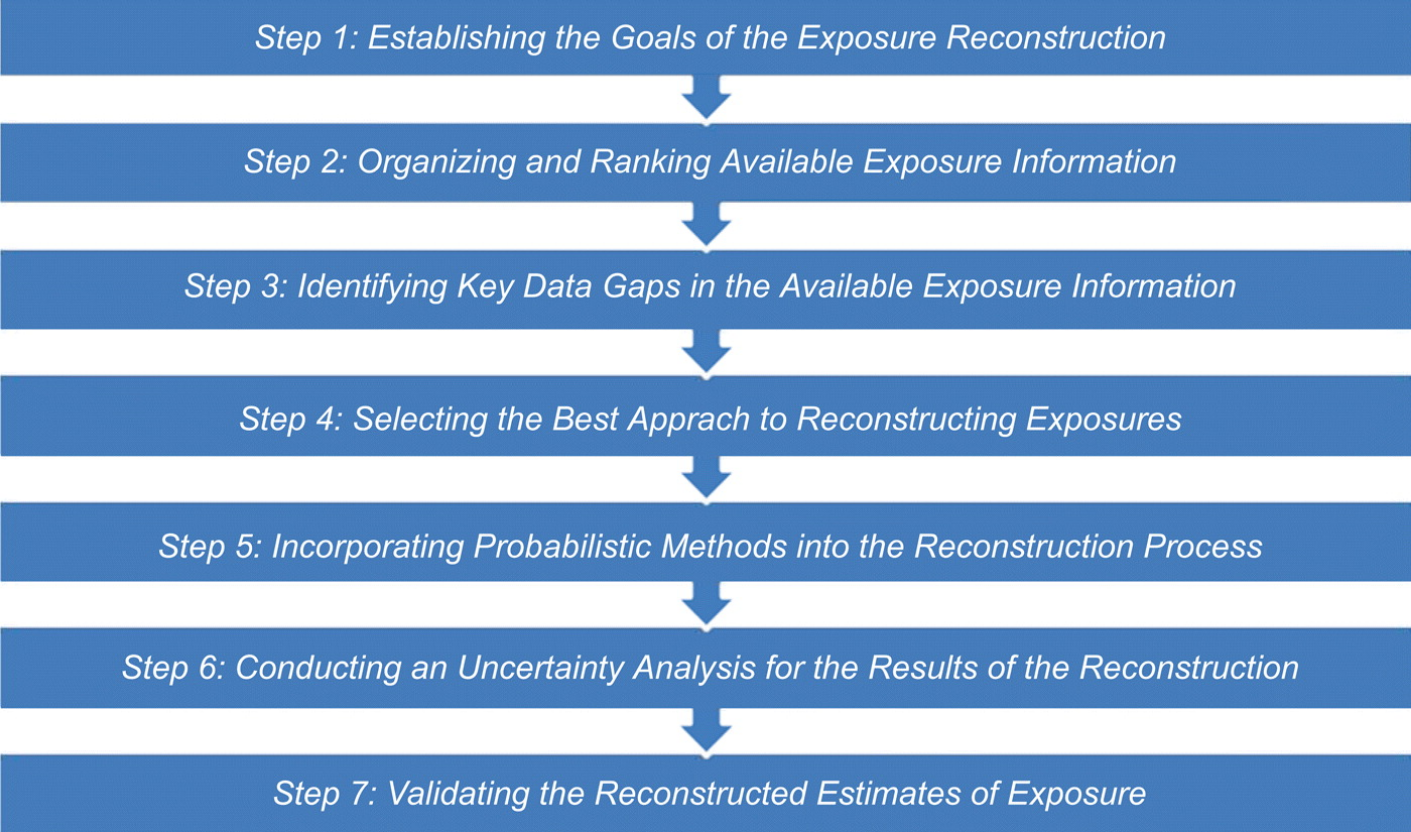
\includegraphics[width=0.5\textwidth,height=\textheight]{./tex2pdf.-c788ce828caea25c/eae30e5bbeba97abd6c389a0e99961dc789fc4a9.png}
\caption{Seven step framework for exposure
reconstruction\label{ssframework}}
\end{figure}

\hypertarget{job-exposure-matrices}{%
\subsubsection{Job-exposure matrices}\label{job-exposure-matrices}}

Several job-exposure matrices that deal with asbestos have been
reported. Pannett et al's 1985 job-exposure matrix for use in population
studies in England and Wales{[}59{]} found good agreement between
job-title assigned categories of exposure (none, low, moderate, high)
for asbestos and direct review of the original occupational history by
an expert.

Rake et al{[}38{]} assigned categories risk of exposure (low, medium,
high) using occupational mortality statistics for pleural mesothelioma.
Because pleural mesothelioma in men is nearly entirely attributable to
occupational asbestos exposure, pleural mesothelioma is rapidly fatal,
and death certificates record occupation in addition to cause of death,
the proportional mortality ratio for pleural mesothelioma (number of
deaths due to pleural mesothelioma/total number of deaths) can serve as
proxy for average asbestos exposure in a particular occupation. This
approach has been validated in the same cohort by amphibole fibre
counts.{[}48{]}

DOM-JEM{[}60{]} was developed for use in population based multi-centre
lung cancer case-control study. It assigns job titles one of three
categories of asbestos exposure (no exposure, low exposure, high
exposure) based on the consensus of three independent expert raters.
DOM-JEM showed poor agreement with expert assessment
(\ensuremath{\kappa = 0.17}) but less heterogeneity. In a study applying
DOM-JEM to the Netherlands Cohort Study (NCS) DOM-JEM showed poor
agreement with expert assessment (K = 0.29).{[}61{]}

The Finish Information System on Occupational Exposure (FINJEM){[}62{]}
covers exposure to 84 different agents, including asbestos, for 311 jobs
across 9 periods spanning 1945-2015. Era-specific estimates of the mean
level of asbestos exposure are available for 27 jobs based on expert
assessment and measurement data; the exact details of the grounds for
estimates are kept in a proprietary FINJEM database which is not freely
available. FINJEM showed poor agreement with expert assessment of
asbestos exposure (\ensuremath{\kappa = 0.23}) but reasonable
identification of mesothelioma risk when evaluated using the
NCS.{[}61{]}{[}63{]}

AsbJEM{[}64{]} was developed in Australia by an expert panel of three
industrial hygienists using all available exposure data. It is based on
FINJEM and provides quantitative estimates of annual exposure for 224
occupations across three time periods spanning 1943 to 2004. It also
showed poor agreement with expert assessment of asbestos exposure
(\ensuremath{\kappa = 0.10})

SYN-JEM{[}65{]} describes a JEM developed for four carcinogens. It
provides quantified asbestos exposure estimates based on 27958 personal
measurements (spanning 1971-2009), a mixed effects statistical model,
and a priori categorical assessment of exposure (none, low, high).
Cherrie et al{[}66{]} point out that SYN-JEM provides little contrast in
the modelled exposure level between categories as the geometric mean for
low jobs was 0.061 fibres/ml and for high jobs 0.074 fibres/ml and that
there are wide variations in regional estimates that are difficult to
explain.

JEMS are generally taken to be superior to direct questions about
exposures because they are cheaper, have greater validity, and are less
vulnerable to differential recall. This is because recall of occupations
is not influenced by disease status, coding of occupation is blind to
case-control status, and translation of codes into exposure is
standardized and can not be influence by disease status of a
subject.{[}67{]}{[}68{]}{[}69{]}

Orlowski et al{[}70{]} compared two JEMs with a structured job specific
questionnaire (SQ) in a lung cancer case-control study. They found that
agreement between the JEMs and the SQ was poor
(\ensuremath{\kappa = 0.23-0.27}) and suggested that the sources of
error for JEMs were loss of information due to the use of job codes as
surrogates for job task descriptions and the insufficiency of published
data on occupational asbestos exposure.

JEMs are not routinely used in clinical practice because they are not
usually available or accessible for specific patients. In a research
setting they are frequently helpful though in addition to the strengths
and weaknesses outlined about the desirability of reusing an existing
JEM vs developing a study specific JEM must be considered.

\hypertarget{exposure-modelling-approaches}{%
\subsubsection{Exposure modelling
approaches}\label{exposure-modelling-approaches}}

Exposure modelling approaches modify existing measurement data on the
basis of knowledge of the determinants of exposure. They may be viewed
as the formalization of professional decision criteria used by
hygienists in their assessment of workplace exposures.{[}55{]}

A common conceptual framework for this is the source-receptor model
source receptor model{[}71{]}{[}55{]} whereby inhalation exposure is
considered in terms of an exposure source, a pathway from source to
receptor, and the receptor. The model is then used to propose modifying
factors such as activity emission potential, substance emission
potential, localized control, worker behavior, surface contamination and
respiratory protection.{[}71{]}.

In the hands of some hygienists assessment of historic asbestos exposure
based on interview can correlate well with amphibole fibre
counts.{[}72{]} By extension, exposure modelling approaches, using
industrial hygienist methods, might be expected to be useful. Exposure
modelling approaches make strong intuitive sense; it is known that there
is significant within-worker and between-worker variability in
occupational exposures{[}73{]} and, for example, room size and
ventilation have been empirically shown to affect the concentration of
airborne chemical exposures.{[}74{]} Further, mathematical exposure
models that take account of known exposure modifying factors to estimate
past exposures have shown a good correlation with measured
values.{[}41{]}

A quantified validated historic asbestos exposure model{[}66{]} has
recently been developed and proposed as a means of for risk stratifying
asbestos exposed workers to optimize mesothelioma screening efforts. The
approach has the advantage, compared with job-exposure matrices, of
providing a more granular quantified exposure assessment, sensitive to
the exposure circumstances of the individual. However, the approach is
limited by the fact that the individual must recall that they must
recall their exposure circumstances which due to the latency of asbestos
related disease may have occurred over 30 years ago. The approach is
also limited by the relatively small number of industry-specific data
points used for validation, though is unavoidable because of the
scarcity of exposure measurement data.

Exposure modelling approaches to assessing asbestos exposure have
research and clinical utility notwithstanding the limitations outlined
above together with the requirement that assessors be appropriately
trained.

\hypertarget{self-reported-exposure}{%
\subsubsection{Self-reported exposure}\label{self-reported-exposure}}

Self-reported exposures are a subjects direct report of what they have
been exposed to. Typically this is elicited by asking about a specific
exposure via questionnaire or interview. Differential recall of
self-reported exposures according to disease status is a concern but few
studies have found evidence of this and it appears to be less of an
issue when prompted responses, rather than volunteered, responses about
occupational exposures are used.{[}75{]}

Most studies comparing self-reported exposures to industrial hygiene
measurements have found significant associations but with wide variation
in the proportions of variance explained by the self reports. This is
not surprising given that it is known there is significant within-worker
and between-worker variability in occupational
exposures.{[}68{]}{[}73{]}

Studies comparing self-reported exposures to expert assessment find
highly variable levels of agreement (\ensuremath{\kappa -0.05 - 0.94})
with a median \ensuremath{\kappa 0.6} . In two studies comparing
self-reported exposures with JEMs, self-reported exposures were more
sensitive and of similar or worse specificity.{[}68{]}

Self-reported exposures have been shown to be more accurate for easily
sensed exposures such as solvents with a strong smell, dusts with larger
particle sizes, and vibrations that can be felt. Providing a reference
point, for example using well known machines from a workplace to gauge
noise category also improves accuracy.{[}68{]}

Self-reported exposures have clinical utility in that they can suggest
or support consideration of an occupational cause for disease. Ideally
such self-reports are combined with the clinicians knowledge of the
likely occupational exposures given the occupational history and other
available data to strengthen or weaken the case as appropriate.
Similarly, they have utility in a research setting where they may
augment other means of assessment.

\hypertarget{discussion-2}{%
\section{Discussion}\label{discussion-2}}

The accuracy of historic asbestos exposure assessment, by any means, is
limited by the paucity of occupational asbestos measurement data,
measurement technique limitations, within and between worker exposure
variability, and participant recall. There does not exist a universally
agreed ``gold standard'' against which to evaluate methods. Accurate
quantified assessment of historic exposure, where evidence is scarce,
may be an impossible task.{[}76{]}

Nonetheless, clinically, historic asbestos exposure assessments must be
made for attribution. Specifically, to inform whether the required
threshold of asbestos exposure (as assessed by various means) has been
crossed so it is possible to say that, for example, scarring of the lung
with an usual interstital pneumonia pattern in an individual patient is
caused by asbestos exposure. This carries medicolegal in addition to
scientific importance and has not been well established by any
assessment method.

In the context of mesothelioma case-control studies fibre-counts do at
least provide an objective means of assessing historic asbestos exposure
against which other means can be compared. It is encouraging that
industrial hygienist assessment and assessment using job title and PMR
correlates strongly with fibre counts.{[}69{]}{[}48{]} Further and more
generally, it is encouraging that estimates from explicit asbestos
exposure modelling systems such as Cherrie et al's{[}66{]}, show good
correlation with measurement data.

\hypertarget{conclusion-2}{%
\section{Conclusion}\label{conclusion-2}}

Quantitative estimates of historic occupational asbestos exposures will
generally have high uncertainty. However, less precise measures, such as
relative difference in exposure among epidemiological groups may be
quite certain even though the numerical estimates are only approximate.
This is invaluable in studies examining aetiological hypothesis.{[}55{]}

\hypertarget{genetic-susceptibility-in-ipf-and-muc5b-muc5b-enivornmental-insult-ipf}{%
\chapter{Genetic susceptibility in IPF and MUC5b: MUC5b + enivornmental
insult =
IPF?}\label{genetic-susceptibility-in-ipf-and-muc5b-muc5b-enivornmental-insult-ipf}}

\hypertarget{introduction-3}{%
\section{Introduction}\label{introduction-3}}

Advances in our understanding of IPF susceptibility now permit study of
host-exposure interactions. The minor-allele of the rs35705950 SNP in
the promotor region of the mucin 5B gene was found to be present in 38\%
of IPF patients but just 9\% of controls.{[}77{]} The polymorphism
results in excess MUC5B protein in the airway, impaired clearance of
inhaled substances and a chronic inflammatory burden on the alveolar
surface.{[}77{]} The association is allele dose-dependent, has been
replicated in independent cohorts, and may affect survival (in what
direction is contested).{[}3{]}{[}77{]}{[}78{]}{[}79{]} Two large GWASs
have confirmed the observed associations of IPF with MUC5B and other
loci.{[}80{]}{[}81{]}

\hypertarget{method-3}{%
\section{Method}\label{method-3}}

We searched pubmed and google scholar for combinations and synonyms of
``asbestos'', ``exposure assessment'', together with terms for modes of
assessment including ``lung biopsy'', ``bronchoalveolar lavage'',
``exposure reconstruction'', and ``job-exposure matrix''. When a
relevant papers was identified, papers referenced, and papers citing,
the paper were reviewed.

\hypertarget{results-3}{%
\section{Results}\label{results-3}}

\hypertarget{discussion-3}{%
\section{Discussion}\label{discussion-3}}

\hypertarget{conclusion-3}{%
\section{Conclusion}\label{conclusion-3}}

\hypertarget{idiopathic-pulmonary-fibrosis-job-exposures-study-ipfjes-is-occupational-asbestos-exposure-an-under-regcognised-cause-of-ipf}{%
\chapter{Idiopathic pulmonary fibrosis job exposures study (IPFJES): Is
occupational asbestos exposure an under-regcognised cause of
IPF?}\label{idiopathic-pulmonary-fibrosis-job-exposures-study-ipfjes-is-occupational-asbestos-exposure-an-under-regcognised-cause-of-ipf}}

\hypertarget{introduction-4}{%
\section{Introduction}\label{introduction-4}}

My study will be a multi-centre, hospital-outpatient, incident
case-control study. Participants will be recruited from a UK network of
six confirmed centres. Cases will be men who present, between 07.2017
and 07.2019, with a new diagnosis of IPF consistent with standard
criteria{[}82{]}; they will be identified monthly by the MDT coordinator
of participating centres.{[}83{]}

For each case, four controls, frequency-matched on age, will be randomly
selected from incident outpatient attendances (not confined to
respiratory) who do not have a diagnosis of IPF and are from the
hospital as the case. Monthly lists of outpatient attendances will be
obtained using the patient administration systems of participating
centres. 120 cases and 480 controls will be recruited over two years
with four participants enrolled and interviewed per day.

Eligible participants will be contacted by telephone and invited to
participate. An interviewer will collect data on demographics, lifetime
occupational history, hobbies, family medical history, and smoking using
a structured web-based questionnaire designed by us to collect lifetime
occupational histories. This approach will facilitate coding, allow
input validation, and permit questions to be tailored to pre-specified
conditions. The questions will be developed in collaboration with an
international expert in asbestos exposure measurement, Dr John Cherrie
of the IOM. Participants will be invited to provide a venous blood
sample for genetic analysis.

Cases and controls will be genotyped using a panel of 15 pre-defined
candidate susceptibility SNPs including rs35705950. Genotyping will be
undertaken using Q-PCR and Taqman assays on DNA isolated from whole
blood samples.

For the primary analysis unconditional logistic regression will be used
to analyse `any' vs `no' asbestos exposure and categories of cumulative
exposure adjusting for age and smoking status. Prior data{[}38{]}
indicate that the probability of exposure among controls is 0.29. If the
true OR for disease in exposed subjects relative to unexposed subjects
is 2.0, I will need to recruit 94 case patients and 376 control patients
to be able to reject the null hypothesis that this odds ratio equals 1
with \ensuremath{\beta = 0.2} and \ensuremath{\alpha = 0.05}{[}84{]}; my
planned sample size sample size includes a margin for model stability
and incomplete data.{[}85{]}

Secondary (exploratory) analysis will investigate gene-environment
interaction. The global minor allele frequency of MUC5B rs35705950 is
0.05.{[}86{]} With an estimated prevalence of IPF of 20/100000{[}1{]}
and with ORs 2.0 for asbestos exposure and 6.8 for rs35705950{[}77{]},
113 cases would be required to detect a minimum interaction OR of
4.0.{[}87{]} While I acknowledge that this exploratory analysis will
have the power to detect only a large effect size it seems a valuable
opportunity to examine an unexplored area in IPF research.

\hypertarget{method-4}{%
\section{Method}\label{method-4}}

In tincidunt viverra dolor, ac pharetra tellus faucibus eget.
Pellentesque tempor a enim nec venenatis. Morbi blandit magna imperdiet
posuere auctor. Maecenas in maximus est.

\hypertarget{results-4}{%
\section{Results}\label{results-4}}

These are the results. Curabitur vulputate nisl non ante tincidunt
tempor. Aenean porta nisi quam, sed ornare urna congue sed. Curabitur in
sapien justo. Quisque pulvinar ullamcorper metus, eu varius mauris
pellentesque et. In hac habitasse platea dictumst. Pellentesque nec
porttitor libero. Duis et magna a massa lacinia cursus.

\hypertarget{discussion-4}{%
\section{Discussion}\label{discussion-4}}

possibility of missed chronic HP {[}88{]}

\hypertarget{conclusion-4}{%
\section{Conclusion}\label{conclusion-4}}

This is the conclusion to the chapter. Nulla sed condimentum lectus.
Duis sed tempor erat, at cursus lacus. Nam vitae tempus arcu, id
vestibulum sapien. Cum sociis natoque penatibus et magnis dis parturient
montes, nascetur ridiculus mus.

\hypertarget{conclusion-5}{%
\chapter{Conclusion}\label{conclusion-5}}

\hypertarget{thesis-summary}{%
\section{Thesis summary}\label{thesis-summary}}

In summary, pellentesque habitant morbi tristique senectus et netus et
malesuada fames ac turpis egestas. Nunc eleifend, ex a luctus porttitor,
felis ex suscipit tellus, ut sollicitudin sapien purus in libero. Nulla
blandit eget urna vel tempus. Praesent fringilla dui sapien, sit amet
egestas leo sollicitudin at.

\hypertarget{future-work}{%
\section{Future work}\label{future-work}}

chronic hp

\hypertarget{appendix-1-ipf-epidemiology-code}{%
\chapter*{Appendix 1: IPF epidemiology
code}\label{appendix-1-ipf-epidemiology-code}}
\addcontentsline{toc}{chapter}{Appendix 1: IPF epidemiology code}

\href{https://github.com/drcjar/pypf}{IPF epidemiology}

\hypertarget{appendix-2-ipfjes-study-documentation}{%
\chapter*{Appendix 2: IPFJES study
documentation}\label{appendix-2-ipfjes-study-documentation}}
\addcontentsline{toc}{chapter}{Appendix 2: IPFJES study documentation}

\href{https://github.com/drcjar/ipfjes/}{IPFJES study documentation}

\footnotesize

\hypertarget{references}{%
\chapter*{References}\label{references}}
\addcontentsline{toc}{chapter}{References}

\hypertarget{refs}{}
\leavevmode\hypertarget{ref-Navaratnam2011}{}%
1 Navaratnam V, Fleming K, West J \emph{et al.} The rising incidence of
idiopathic pulmonary fibrosis in the uk. \emph{Thorax}
2011;\textbf{66}:462--7.

\leavevmode\hypertarget{ref-Maher2012}{}%
2 Maher TM. Idiopathic pulmonary fibrosis: Pathobiology of novel
approaches to treatment. \emph{Clin Chest Med} 2012;\textbf{33}:69--83.
doi:\href{https://doi.org/10.1016/j.ccm.2011.11.002}{10.1016/j.ccm.2011.11.002}

\leavevmode\hypertarget{ref-Ley2013}{}%
3 Ley B, Collard HR. Epidemiology of idiopathic pulmonary fibrosis.
\emph{Clinical epidemiology} 2013;\textbf{5}:483.

\leavevmode\hypertarget{ref-Spagnolo2014}{}%
4 Spagnolo P, Grunewald J, Bois RM du. Genetic determinants of pulmonary
fibrosis: Evolving concepts. \emph{The Lancet Respiratory Medicine}
2014;\textbf{2}:416--28.

\leavevmode\hypertarget{ref-Hubbard1998}{}%
5 Hubbard R, Johnston I, Britton J. Survival in patients with
cryptogenic fibrosing alveolitis a population-based cohort study.
\emph{CHEST Journal} 1998;\textbf{113}:396--400.

\leavevmode\hypertarget{ref-Vancheri2010}{}%
6 Vancheri C, Failla M, Crimi N \emph{et al.} Idiopathic pulmonary
fibrosis: A disease with similarities and links to cancer biology.
\emph{Eur Respir J} 2010;\textbf{35}:496--504.
doi:\href{https://doi.org/10.1183/09031936.00077309}{10.1183/09031936.00077309}

\leavevmode\hypertarget{ref-Barber2015}{}%
7 Barber C, Wiggans R, Young C \emph{et al.} UK asbestos imports and
mortality due to idiopathic pulmonary fibrosis. \emph{Occup Med}
2015;kqv142.

\leavevmode\hypertarget{ref-Monso1990}{}%
8 Monso E, Tura JM, Marsal M \emph{et al.} Mineralogical microanalysis
of idiopathic pulmonary fibrosis. \emph{Arch Environ Health}
1990;\textbf{45}:185--8.
doi:\href{https://doi.org/10.1080/00039896.1990.9936714}{10.1080/00039896.1990.9936714}

\leavevmode\hypertarget{ref-Monso1991}{}%
9 Monsó E, Tura J, Pujadas J \emph{et al.} Lung dust content in
idiopathic pulmonary fibrosis: A study with scanning electron microscopy
and energy dispersive x ray analysis. \emph{Br J Ind Med}
1991;\textbf{48}:327--31.

\leavevmode\hypertarget{ref-Glazer2009}{}%
10 Glazer C, Maier L. Occupational interstitial lung disease. \emph{Eur
Respir Monograph} 2009;\textbf{46}:265--86.

\leavevmode\hypertarget{ref-Ghio2014}{}%
11 Ghio A, Sangani R, Roggli V. Expanding the spectrum of particle-and
fiber-associated interstitial lung diseases. \emph{Turk Toraks Derg}
2014;\textbf{15}:1--8.

\leavevmode\hypertarget{ref-Travis2013}{}%
12 Travis WD, Costabel U, Hansell DM \emph{et al.} An official american
thoracic society/european respiratory society statement: Update of the
international multidisciplinary classification of the idiopathic
interstitial pneumonias. \emph{American journal of respiratory and
critical care medicine} 2013;\textbf{188}:733--48.

\leavevmode\hypertarget{ref-Reynolds2017}{}%
13 Reynolds CJ, Blanc PD. Organising pneumonia and other uncommon
interstitial disorders. In: \emph{Parkes' occupational lung disorders,
fourth edition}. 2018.

\leavevmode\hypertarget{ref-Turner-Warwick1998}{}%
14 Turner-Warwick M. In search of a cause of cryptogenic fibrosing
alveolitis (cfa): One initiating factor or many? \emph{Thorax}
1998;\textbf{53}:S3--9.

\leavevmode\hypertarget{ref-Hubbard2001}{}%
15 Hubbard R. Occupational dust exposure and the aetiology of
cryptogenic fibrosing alveolitis. \emph{Eur Respir J}
2001;\textbf{18}:119s--21s.

\leavevmode\hypertarget{ref-Taskar2006}{}%
16 Taskar VS, Coultas DB. Is idiopathic pulmonary fibrosis an
environmental disease? \emph{Proc Am Thorac Soc} 2006;\textbf{3}:293--8.

\leavevmode\hypertarget{ref-Gulati2015}{}%
17 Gulati M, Redlich CA. Asbestosis and environmental causes of usual
interstitial pneumonia. \emph{Current opinion in pulmonary medicine}
2015;\textbf{21}:193--200.
doi:\href{https://doi.org/10.1097/MCP.0000000000000144}{10.1097/MCP.0000000000000144}

\leavevmode\hypertarget{ref-Fontaine2009}{}%
18 Fontaine J-F, Barbosa-Silva A, Schaefer M \emph{et al.}
MedlineRanker: Flexible ranking of biomedical literature. \emph{Nucleic
acids research} 2009;\textbf{37}:W141--6.
doi:\href{https://doi.org/10.1093/nar/gkp353}{10.1093/nar/gkp353}

\leavevmode\hypertarget{ref-Reynolds2017pubmed}{}%
19 Reynolds C, De Matteis S, Cullinan P \emph{et al.} Pubmed mining for
occupational idiopathic pulmonary fibrosis papers. 2017.

\leavevmode\hypertarget{ref-Scott1990}{}%
20 Scott J, Johnston I, Britton J. What causes cryptogenic fibrosing
alveolitis? A case-control study of environmental exposure to dust.
\emph{BMJ} 1990;\textbf{301}:1015.

\leavevmode\hypertarget{ref-Iwai1994}{}%
21 Iwai K, Mori T, Yamada N \emph{et al.} Idiopathic pulmonary fibrosis.
Epidemiologic approaches to occupational exposure. \emph{Am J Respir
Crit Care Med} 1994;\textbf{150}:670--5.
doi:\href{https://doi.org/10.1164/ajrccm.150.3.8087336}{10.1164/ajrccm.150.3.8087336}

\leavevmode\hypertarget{ref-Hubbard1996a}{}%
22 Hubbard R, Lewis S, Richards K \emph{et al.} Occupational exposure to
metal or wood dust and aetiology of cryptogenic fibrosing alveolitis.
\emph{The Lancet} 1996;\textbf{347}:284--9.

\leavevmode\hypertarget{ref-Mullen1998}{}%
23 Mullen J, Hodgson MJ, DeGraff CA \emph{et al.} Case-control study of
idiopathic pulmonary fibrosis and environmental exposures. \emph{J Occup
Environ Med} 1998;\textbf{40}:363--7.

\leavevmode\hypertarget{ref-Baumgartner2000}{}%
24 Baumgartner KB, Samet JM, Coultas DB \emph{et al.} Occupational and
environmental risk factors for idiopathic pulmonary fibrosis: A
multicenter case-control study. Collaborating centers. \emph{Am J
Epidemiol} 2000;\textbf{152}:307--15.

\leavevmode\hypertarget{ref-Hubbard2000}{}%
25 Hubbard R, Cooper M, Antoniak M \emph{et al.} Risk of cryptogenic
fibrosing alveolitis in metal workers. \emph{The Lancet}
2000;\textbf{355}:466--7.

\leavevmode\hypertarget{ref-Miyake2005}{}%
26 Miyake Y, Sasaki S, Yokoyama T \emph{et al.} Occupational and
environmental factors and idiopathic pulmonary fibrosis in japan.
\emph{Ann Occup Hyg} 2005;\textbf{49}:259--65.

\leavevmode\hypertarget{ref-Gustafson2007}{}%
27 Gustafson T, Dahlman-Höglund A, Nilsson K \emph{et al.} Occupational
exposure and severe pulmonary fibrosis. \emph{Respir Med}
2007;\textbf{101}:2207--12.

\leavevmode\hypertarget{ref-Pinheiro2008}{}%
28 Pinheiro GA, Antao VC, Wood JM \emph{et al.} Occupational risks for
idiopathic pulmonary fibrosis mortality in the united states. \emph{Int
J Occup Environ Health} 2008;\textbf{14}:117--23.

\leavevmode\hypertarget{ref-Garcia-SanchoFigueroa2010}{}%
29 García-Sancho Figueroa MC, Carrillo G, Pérez-Padilla R \emph{et al.}
Risk factors for idiopathic pulmonary fibrosis in a mexican population.
A case-control study. \emph{Respir Med} 2010;\textbf{104}:305--9.

\leavevmode\hypertarget{ref-Garcia-Sancho2011}{}%
30 García-Sancho C, Buendía-Roldán I, Fernández-Plata MR \emph{et al.}
Familial pulmonary fibrosis is the strongest risk factor for idiopathic
pulmonary fibrosis. \emph{Respiratory medicine}
2011;\textbf{105}:1902--7.
doi:\href{https://doi.org/10.1016/j.rmed.2011.08.022}{10.1016/j.rmed.2011.08.022}

\leavevmode\hypertarget{ref-Awadalla2012}{}%
31 Awadalla NJ, Hegazy A, Elmetwally RA \emph{et al.} Occupational and
environmental risk factors for idiopathic pulmonary fibrosis in egypt: A
multicenter case-control study. \emph{Int J Occup Environ Med}
2012;\textbf{3}:107--16.

\leavevmode\hypertarget{ref-Paolocci2013}{}%
32 Paolocci G, Nicolic V, Folletti I \emph{et al.} Risk factors for
idiopathic pulmonary fibrosis in southern europe: A case-control study.
2013.

\leavevmode\hypertarget{ref-Ekstrom2014}{}%
33 Ekstrom M, Gustafson T, Boman K \emph{et al.} Effects of smoking,
gender and occupational exposure on the risk of severe pulmonary
fibrosis: A population-based case-control study. \emph{BMJ open}
2014;\textbf{4}:e004018.

\leavevmode\hypertarget{ref-Koo2017}{}%
34 Koo J-W, Myong J-P, Yoon H-K \emph{et al.} Occupational exposure and
idiopathic pulmonary fibrosis: A multicentre case-control study in
korea. \emph{The international journal of tuberculosis and lung disease
: the official journal of the International Union against Tuberculosis
and Lung Disease} 2017;\textbf{21}:107--12.
doi:\href{https://doi.org/10.5588/ijtld.16.0167}{10.5588/ijtld.16.0167}

\leavevmode\hypertarget{ref-Hubbard1996}{}%
35 Hubbard R, Johnston I, Coultas DB \emph{et al.} Mortality rates from
cryptogenic fibrosing alveolitis in seven countries. \emph{Thorax}
1996;\textbf{51}:711--6.

\leavevmode\hypertarget{ref-Navaratnam2014}{}%
36 Navaratnam V, Fogarty AW, McKeever T \emph{et al.} Presence of a
prothrombotic state in people with idiopathic pulmonary fibrosis: A
population-based case-control study. \emph{Thorax}
2014;\textbf{69}:207--15.
doi:\href{https://doi.org/10.1136/thoraxjnl-2013-203740}{10.1136/thoraxjnl-2013-203740}

\leavevmode\hypertarget{ref-Welch1994}{}%
37 Welch LS, Michaels D, Zoloth SR. The national sheet metal worker
asbestos disease screening program: Radiologic findings. National sheet
metal examination group. \emph{Am J Ind Med} 1994;\textbf{25}:635--48.

\leavevmode\hypertarget{ref-Rake2009}{}%
38 Rake C, Gilham C, Hatch J \emph{et al.} Occupational, domestic and
environmental mesothelioma risks in the british population: A
case-control study. \emph{Br J Cancer} 2009;\textbf{100}:1175--83.
doi:\href{https://doi.org/10.1038/sj.bjc.6604879}{10.1038/sj.bjc.6604879}

\leavevmode\hypertarget{ref-Caminati2015}{}%
39 Caminati A, Madotto F, Cesana G \emph{et al.} Epidemiological studies
in idiopathic pulmonary fibrosis: Pitfalls in methodologies and data
interpretation. \emph{European respiratory review : an official journal
of the European Respiratory Society} 2015;\textbf{24}:436--44.
doi:\href{https://doi.org/10.1183/16000617.0040-2015}{10.1183/16000617.0040-2015}

\leavevmode\hypertarget{ref-DeVuyst1998}{}%
40 De Vuyst P, Karjalainen A, Dumortier P \emph{et al.} Guidelines for
mineral fibre analyses in biological samples: Report of the ers working
group. European respiratory society. \emph{The European respiratory
journal} 1998;\textbf{11}:1416--26.

\leavevmode\hypertarget{ref-Cherrie1999}{}%
41 Cherrie JW, Schneider T. Validation of a new method for structured
subjective assessment of past concentrations. \emph{Ann Occup Hyg}
1999;\textbf{43}:235--45.

\leavevmode\hypertarget{ref-Nemery2017}{}%
42 Nemery B, Nuyts V, Nackaerts K. Quantifying asbestos in lung tissue:
What debate? \emph{The European respiratory journal} 2017;\textbf{49}.
doi:\href{https://doi.org/10.1183/13993003.00861-2017}{10.1183/13993003.00861-2017}

\leavevmode\hypertarget{ref-Cooke1924}{}%
43 Cooke WE. FIBROSIS of the lungs due to the inhalation of asbestos
dust. \emph{British medical journal} 1924;\textbf{2}:147--140.2.

\leavevmode\hypertarget{ref-Wolff2015}{}%
44 Wolff H, Vehmas T, Oksa P \emph{et al.} Asbestos, asbestosis, and
cancer, the helsinki criteria for diagnosis and attribution 2014:
Recommendations. \emph{Scandinavian journal of work, environment \&
health} 2015;\textbf{41}:5--15.
doi:\href{https://doi.org/10.5271/sjweh.3462}{10.5271/sjweh.3462}

\leavevmode\hypertarget{ref-Hammar2015}{}%
45 Hammar SP, Abraham JL. Commentary on pathologic diagnosis of
asbestosis and critique of the 2010 asbestosis committee of the college
of american pathologists (cap) and pulmonary pathology society's (pps)
update on the diagnostic criteria for pathologic asbestosis.
\emph{American journal of industrial medicine} 2015;\textbf{58}:1034--9.
doi:\href{https://doi.org/10.1002/ajim.22512}{10.1002/ajim.22512}

\leavevmode\hypertarget{ref-Baur2016}{}%
46 Baur X, Frank AL, Budnik LT \emph{et al.} Collegium ramazzini:
Comments on the 2014 helsinki consensus report on asbestos.
\emph{American journal of industrial medicine} 2016;\textbf{59}:591--4.
doi:\href{https://doi.org/10.1002/ajim.22595}{10.1002/ajim.22595}

\leavevmode\hypertarget{ref-Baur2017}{}%
47 Baur X, Woitowitz H-J, Budnik LT \emph{et al.} Asbestos, asbestosis,
and cancer: The helsinki criteria for diagnosis and attribution.
Critical need for revision of the 2014 update. \emph{American journal of
industrial medicine} 2017;\textbf{60}:411--21.
doi:\href{https://doi.org/10.1002/ajim.22709}{10.1002/ajim.22709}

\leavevmode\hypertarget{ref-Gilham2016}{}%
48 Gilham C, Rake C, Burdett G \emph{et al.} Pleural mesothelioma and
lung cancer risks in relation to occupational history and asbestos lung
burden. \emph{Occupational and environmental medicine}
2016;\textbf{73}:290--9.
doi:\href{https://doi.org/10.1136/oemed-2015-103074}{10.1136/oemed-2015-103074}

\leavevmode\hypertarget{ref-Gilham2018}{}%
49 Gilham C, Rake C, Hodgson J \emph{et al.} Past and current asbestos
exposure and future mesothelioma risks in britain: The inhaled particles
study (tips). \emph{International Journal of Epidemiology} 2018.

\leavevmode\hypertarget{ref-Nuyts2017}{}%
50 Nuyts V, Vanhooren H, Begyn S \emph{et al.} Asbestos bodies in
bronchoalveolar lavage in the 21st century: A time-trend analysis in a
clinical population. \emph{Occupational and environmental medicine}
2017;\textbf{74}:59--65.
doi:\href{https://doi.org/10.1136/oemed-2016-103710}{10.1136/oemed-2016-103710}

\leavevmode\hypertarget{ref-Burns1989}{}%
51 Burns D, Beaumont P. The hse national exposure database---(nedb).
\emph{The Annals of occupational hygiene} 1989;\textbf{33}:1--14.

\leavevmode\hypertarget{ref-Orlowski2015}{}%
52 Orlowski E, Audignon-Durand S, Goldberg M \emph{et al.} EV@LUTIL: An
open access database on occupational exposures to asbestos and man-made
mineral fibres. \emph{American journal of industrial medicine}
2015;\textbf{58}:1059--74.
doi:\href{https://doi.org/10.1002/ajim.22498}{10.1002/ajim.22498}

\leavevmode\hypertarget{ref-Peto1985}{}%
53 Peto J. Problems in dose response and risk assessment: The example of
asbestos. In: \emph{Epidemiology and quantitation of environmental risk
in humans from radiation and other agents}. Springer 1985. 175--85.

\leavevmode\hypertarget{ref-ATSDR2001}{}%
54 Toxic Substances A for, (ATSDR). DR. Agency for toxic substances and
disease registry (atsdr). 2001. Toxicological profile for asbestos. U.S.
Department of Health; Human Services, Public Health Service. 2001.
\url{https://www.atsdr.cdc.gov/toxprofiles/TP.asp?id=30\&tid=4\#bookmark16}

\leavevmode\hypertarget{ref-Smith1991}{}%
55 Smith TJ, Hammond SK, Hallock M \emph{et al.} Exposure assessment for
epidemiology: Characteristics of exposure. \emph{Applied Occupational
and Environmental Hygiene} 1991;\textbf{6}:441--7.

\leavevmode\hypertarget{ref-Sahmel2010}{}%
56 Sahmel J, Devlin K, Paustenbach D \emph{et al.} The role of exposure
reconstruction in occupational human health risk assessment: Current
methods and a recommended framework. \emph{Critical reviews in
toxicology} 2010;\textbf{40}:799--843.
doi:\href{https://doi.org/10.3109/10408444.2010.501052}{10.3109/10408444.2010.501052}

\leavevmode\hypertarget{ref-Blake2006}{}%
57 Blake CL, Dotson GS, Harbison RD. Assessment of airborne asbestos
exposure during the servicing and handling of automobile
asbestos-containing gaskets. \emph{Regulatory toxicology and
pharmacology : RTP} 2006;\textbf{45}:214--22.
doi:\href{https://doi.org/10.1016/j.yrtph.2006.04.007}{10.1016/j.yrtph.2006.04.007}

\leavevmode\hypertarget{ref-Williams2007}{}%
58 Williams PRD, Phelka AD, Paustenbach DJ. A review of historical
exposures to asbestos among skilled craftsmen (1940-2006). \emph{Journal
of toxicology and environmental health Part B, Critical reviews}
2007;\textbf{10}:319--77.
doi:\href{https://doi.org/10.1080/10937400601034191}{10.1080/10937400601034191}

\leavevmode\hypertarget{ref-Pannett1985}{}%
59 Pannett B, Coggon D, Acheson ED. A job-exposure matrix for use in
population based studies in england and wales. \emph{British journal of
industrial medicine} 1985;\textbf{42}:777--83.

\leavevmode\hypertarget{ref-Peters2011}{}%
60 Peters S, Vermeulen R, Cassidy A \emph{et al.} Comparison of exposure
assessment methods for occupational carcinogens in a multi-centre lung
cancer case-control study. \emph{Occupational and environmental
medicine} 2011;\textbf{68}:148--53.
doi:\href{https://doi.org/10.1136/oem.2010.055608}{10.1136/oem.2010.055608}

\leavevmode\hypertarget{ref-Offermans2012}{}%
61 Offermans NSM, Vermeulen R, Burdorf A \emph{et al.} Comparison of
expert and job-exposure matrix-based retrospective exposure assessment
of occupational carcinogens in the netherlands cohort study.
\emph{Occupational and environmental medicine} 2012;\textbf{69}:745--51.
doi:\href{https://doi.org/10.1136/oemed-2011-100556}{10.1136/oemed-2011-100556}

\leavevmode\hypertarget{ref-Kauppinen1998}{}%
62 Kauppinen T, Toikkanen J, Pukkala E. From cross-tabulations to
multipurpose exposure information systems: A new job-exposure matrix.
\emph{American journal of industrial medicine} 1998;\textbf{33}:409--17.

\leavevmode\hypertarget{ref-Offermans2014}{}%
63 Offermans NSM, Vermeulen R, Burdorf A \emph{et al.} Occupational
asbestos exposure and risk of pleural mesothelioma, lung cancer, and
laryngeal cancer in the prospective netherlands cohort study.
\emph{Journal of occupational and environmental medicine}
2014;\textbf{56}:6--19.
doi:\href{https://doi.org/10.1097/JOM.0000000000000060}{10.1097/JOM.0000000000000060}

\leavevmode\hypertarget{ref-Oyen2015}{}%
64 Oyen SC van, Peters S, Alfonso H \emph{et al.} Development of a
job-exposure matrix (asbjem) to estimate occupational exposure to
asbestos in australia. \emph{The Annals of occupational hygiene}
2015;\textbf{59}:737--48.
doi:\href{https://doi.org/10.1093/annhyg/mev017}{10.1093/annhyg/mev017}

\leavevmode\hypertarget{ref-Peters2016}{}%
65 Peters S, Vermeulen R, Portengen L \emph{et al.} SYN-jem: A
quantitative job-exposure matrix for five lung carcinogens. \emph{The
Annals of occupational hygiene} 2016;\textbf{60}:795--811.
doi:\href{https://doi.org/10.1093/annhyg/mew034}{10.1093/annhyg/mew034}

\leavevmode\hypertarget{ref-Cherrie2018}{}%
66 Cherrie JW, McElvenny D, Blyth KG. Estimating past inhalation
exposure to asbestos: A tool for risk attribution and disease screening.
\emph{International journal of hygiene and environmental health}
2018;\textbf{221}:27--32.
doi:\href{https://doi.org/10.1016/j.ijheh.2017.09.013}{10.1016/j.ijheh.2017.09.013}

\leavevmode\hypertarget{ref-Ahrens1993}{}%
67 Ahrens W, Jöckel KH, Brochard P \emph{et al.} Retrospective
assessment of asbestos exposure--i. Case-control analysis in a study of
lung cancer: Efficiency of job-specific questionnaires and job exposure
matrices. \emph{International journal of epidemiology} 1993;\textbf{22
Suppl 2}:S83--95.

\leavevmode\hypertarget{ref-Teschke2002}{}%
68 Teschke K, Olshan AF, Daniels JL \emph{et al.} Occupational exposure
assessment in case-control studies: Opportunities for improvement.
\emph{Occup Environ Med} 2002;\textbf{59}:575--93; discussion 594.

\leavevmode\hypertarget{ref-Gramond2012}{}%
69 Gramond C, Rolland P, Lacourt A \emph{et al.} Choice of rating method
for assessing occupational asbestos exposure: Study for compensation
purposes in france. \emph{Am J Ind Med} 2012;\textbf{55}:440--9.
doi:\href{https://doi.org/10.1002/ajim.22008}{10.1002/ajim.22008}

\leavevmode\hypertarget{ref-Orlowski1993}{}%
70 Orlowski E, Pohlabeln H, Berrino F \emph{et al.} Retrospective
assessment of asbestos exposure--ii. At the job level: Complementarity
of job-specific questionnaire and job exposure matrices.
\emph{International journal of epidemiology} 1993;\textbf{22 Suppl
2}:S96--105.

\leavevmode\hypertarget{ref-Tielemans2008}{}%
71 Tielemans E, Schneider T, Goede H \emph{et al.} Conceptual model for
assessment of inhalation exposure: Defining modifying factors. \emph{The
Annals of occupational hygiene} 2008;\textbf{52}:577--86.
doi:\href{https://doi.org/10.1093/annhyg/men059}{10.1093/annhyg/men059}

\leavevmode\hypertarget{ref-Rodelsperger2001}{}%
72 Rödelsperger K, Jöckel KH, Pohlabeln H \emph{et al.} Asbestos and
man-made vitreous fibers as risk factors for diffuse malignant
mesothelioma: Results from a german hospital-based case-control study.
\emph{American journal of industrial medicine} 2001;\textbf{39}:262--75.

\leavevmode\hypertarget{ref-Symanski2006}{}%
73 Symanski E, Maberti S, Chan W. A meta-analytic approach for
characterizing the within-worker and between-worker sources of variation
in occupational exposure. \emph{The Annals of occupational hygiene}
2006;\textbf{50}:343--57.
doi:\href{https://doi.org/10.1093/annhyg/mel006}{10.1093/annhyg/mel006}

\leavevmode\hypertarget{ref-Cherrie1999a}{}%
74 Cherrie JW. The effect of room size and general ventilation on the
relationship between near and far-field concentrations. \emph{Applied
occupational and environmental hygiene} 1999;\textbf{14}:539--46.
doi:\href{https://doi.org/10.1080/104732299302530}{10.1080/104732299302530}

\leavevmode\hypertarget{ref-Teschke2000}{}%
75 Teschke K, Smith JC, Olshan AF. Evidence of recall bias in
volunteered vs. Prompted responses about occupational exposures.
\emph{American journal of industrial medicine} 2000;\textbf{38}:385--8.

\leavevmode\hypertarget{ref-Burstyn2011}{}%
76 Burstyn I. The ghost of methods past: Exposure assessment versus
job-exposure matrix studies. \emph{Occup Environ Med}
2011;\textbf{68}:2--3.
doi:\href{https://doi.org/10.1136/oem.2009.054585}{10.1136/oem.2009.054585}

\leavevmode\hypertarget{ref-Seibold2011}{}%
77 Seibold MA, Wise AL, Speer MC \emph{et al.} A common muc5b promoter
polymorphism and pulmonary fibrosis. \emph{N Engl J Med}
2011;\textbf{364}:1503--12.
doi:\href{https://doi.org/10.1056/NEJMoa1013660}{10.1056/NEJMoa1013660}

\leavevmode\hypertarget{ref-Peljto2013}{}%
78 Peljto AL, Zhang Y, Fingerlin TE \emph{et al.} Association between
the muc5b promoter polymorphism and survival in patients with idiopathic
pulmonary fibrosis. \emph{JAMA} 2013;\textbf{309}:2232--9.

\leavevmode\hypertarget{ref-Dudbridge2019}{}%
79 Dudbridge F, Allen RJ, Sheehan NA \emph{et al.} Adjustment for index
event bias in genome-wide association studies of subsequent events.
\emph{Nature communications} 2019;\textbf{10}:1561.
doi:\href{https://doi.org/10.1038/s41467-019-09381-w}{10.1038/s41467-019-09381-w}

\leavevmode\hypertarget{ref-Fingerlin2013}{}%
80 Fingerlin TE, Murphy E, Zhang W \emph{et al.} Genome-wide association
study identifies multiple susceptibility loci for pulmonary fibrosis.
\emph{Nat Genet} 2013;\textbf{45}:613--20.
doi:\href{https://doi.org/10.1038/ng.2609}{10.1038/ng.2609}

\leavevmode\hypertarget{ref-Noth2013}{}%
81 Noth I, Zhang Y, Ma S-F \emph{et al.} Genetic variants associated
with idiopathic pulmonary fibrosis susceptibility and mortality: A
genome-wide association study. \emph{Lancet Respir Med}
2013;\textbf{1}:309--17.
doi:\href{https://doi.org/10.1016/S2213-2600(13)70045-6}{10.1016/S2213-2600(13)70045-6}

\leavevmode\hypertarget{ref-Raghu2011}{}%
82 Raghu. An official ATS/ERS/JRS/ALAT statement: idiopathic pulmonary
fibrosis: evidence-based guidelines for diagnosis and management,
author=Raghu, Ganesh and Collard, Harold R and Egan, Jim J and Martinez,
Fernando J and Behr, Juergen and Brown, Kevin K and Colby, Thomas V and
Cordier, Jean-François and Flaherty, Kevin R and Lasky, Joseph A and
others. \emph{Am J Respir Crit Care Med} 2011;\textbf{183}:788--824.

\leavevmode\hypertarget{ref-NICE2013}{}%
83 NICE. Idiopathic pulmonary fibrosis: The diagnosis and management of
suspected idiopathic pulmonary fibrosis.
2013.\url{https://www.nice.org.uk/guidance/cg163}

\leavevmode\hypertarget{ref-Dupont1990}{}%
84 Dupont WD, Plummer WD. Power and sample size calculations: A review
and computer program. \emph{Control Clin Trials}
1990;\textbf{11}:116--28.

\leavevmode\hypertarget{ref-Agresti2007}{}%
85 Agresti A. Building and applying logistic regression models.
\emph{Categorical Data Analysis, Second Edition} 2007;211--66.

\leavevmode\hypertarget{ref-Cariaso2012}{}%
86 Cariaso M, Lennon G. SNPedia: A wiki supporting personal genome
annotation, interpretation and analysis. \emph{Nucleic Acids Res}
2012;\textbf{40}:D1308--12.
doi:\href{https://doi.org/10.1093/nar/gkr798}{10.1093/nar/gkr798}

\leavevmode\hypertarget{ref-Gauderman2002}{}%
87 Gauderman WJ. Sample size requirements for association studies of
gene-gene interaction. \emph{Am J Epidemiol} 2002;\textbf{155}:478--84.

\leavevmode\hypertarget{ref-Morell2013}{}%
88 Morell F, Villar A, Montero M-Á \emph{et al.} Chronic
hypersensitivity pneumonitis in patients diagnosed with idiopathic
pulmonary fibrosis: A prospective case-cohort study. \emph{Lancet Respir
Med} 2013;\textbf{1}:685--94.
doi:\href{https://doi.org/10.1016/S2213-2600(13)70191-7}{10.1016/S2213-2600(13)70191-7}

\end{document}
